\chapter{\label{ch8-onsky}On-Sky Observations} 

\minitoc

\section{Introduction}

\begin{figure}
  \centering
  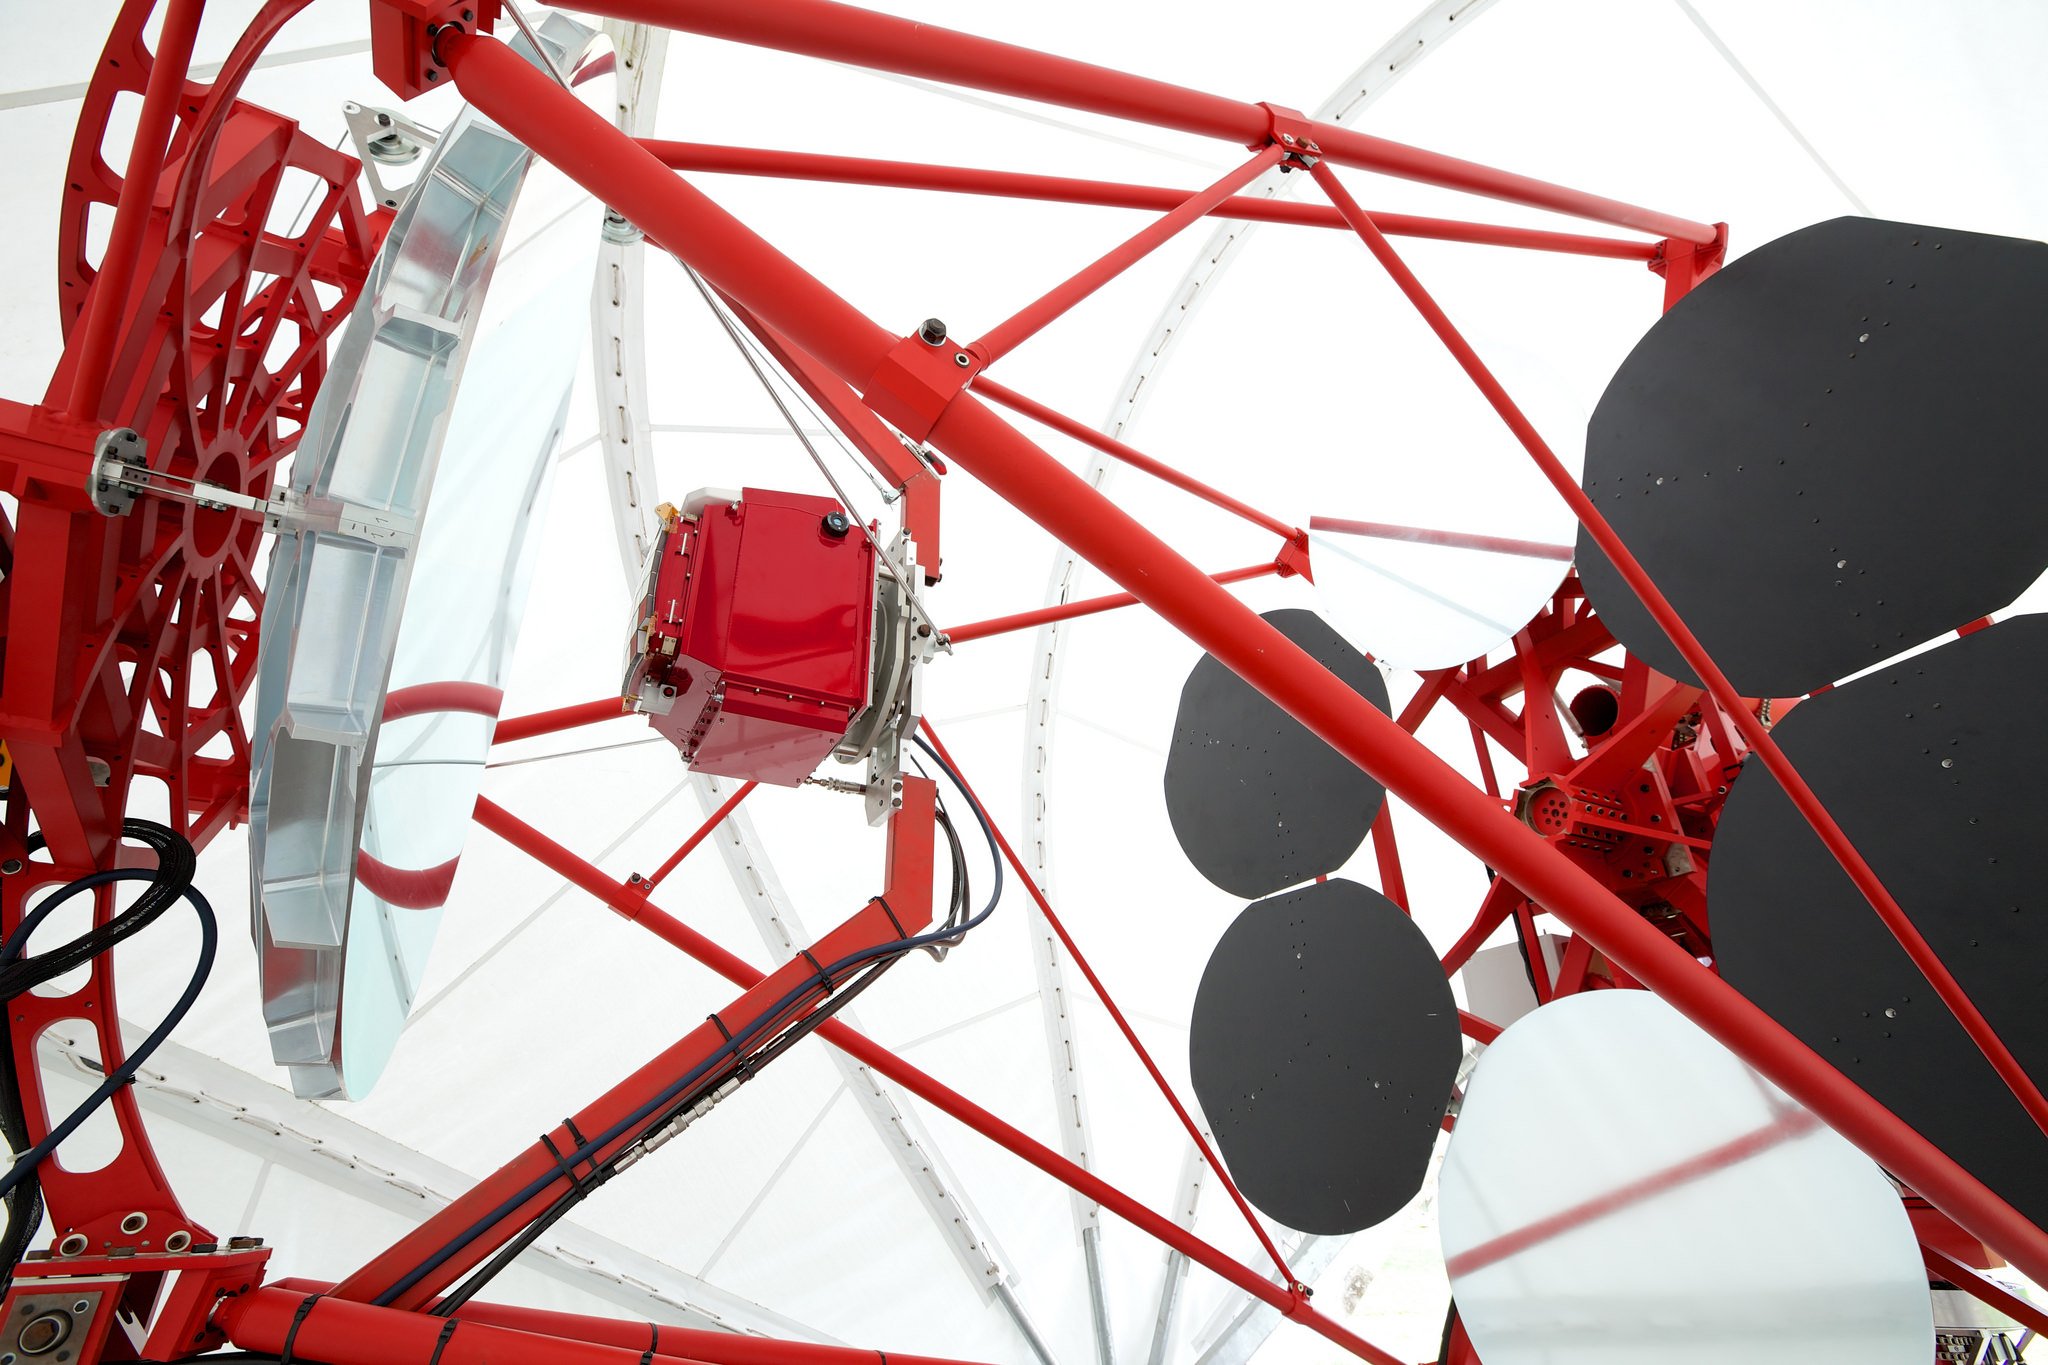
\includegraphics[width=0.8\textwidth]{akira-telescope}
  \caption[Photo of CHEC-M installed on the GCT telescope structure.]{Photo of CHEC-M installed on the GCT telescope structure, taken during the first on-telescope campaign \cite{akira-telescope}.}
  \label{fig:akira-telescope}
\end{figure}

\begin{figure}
  \centering
  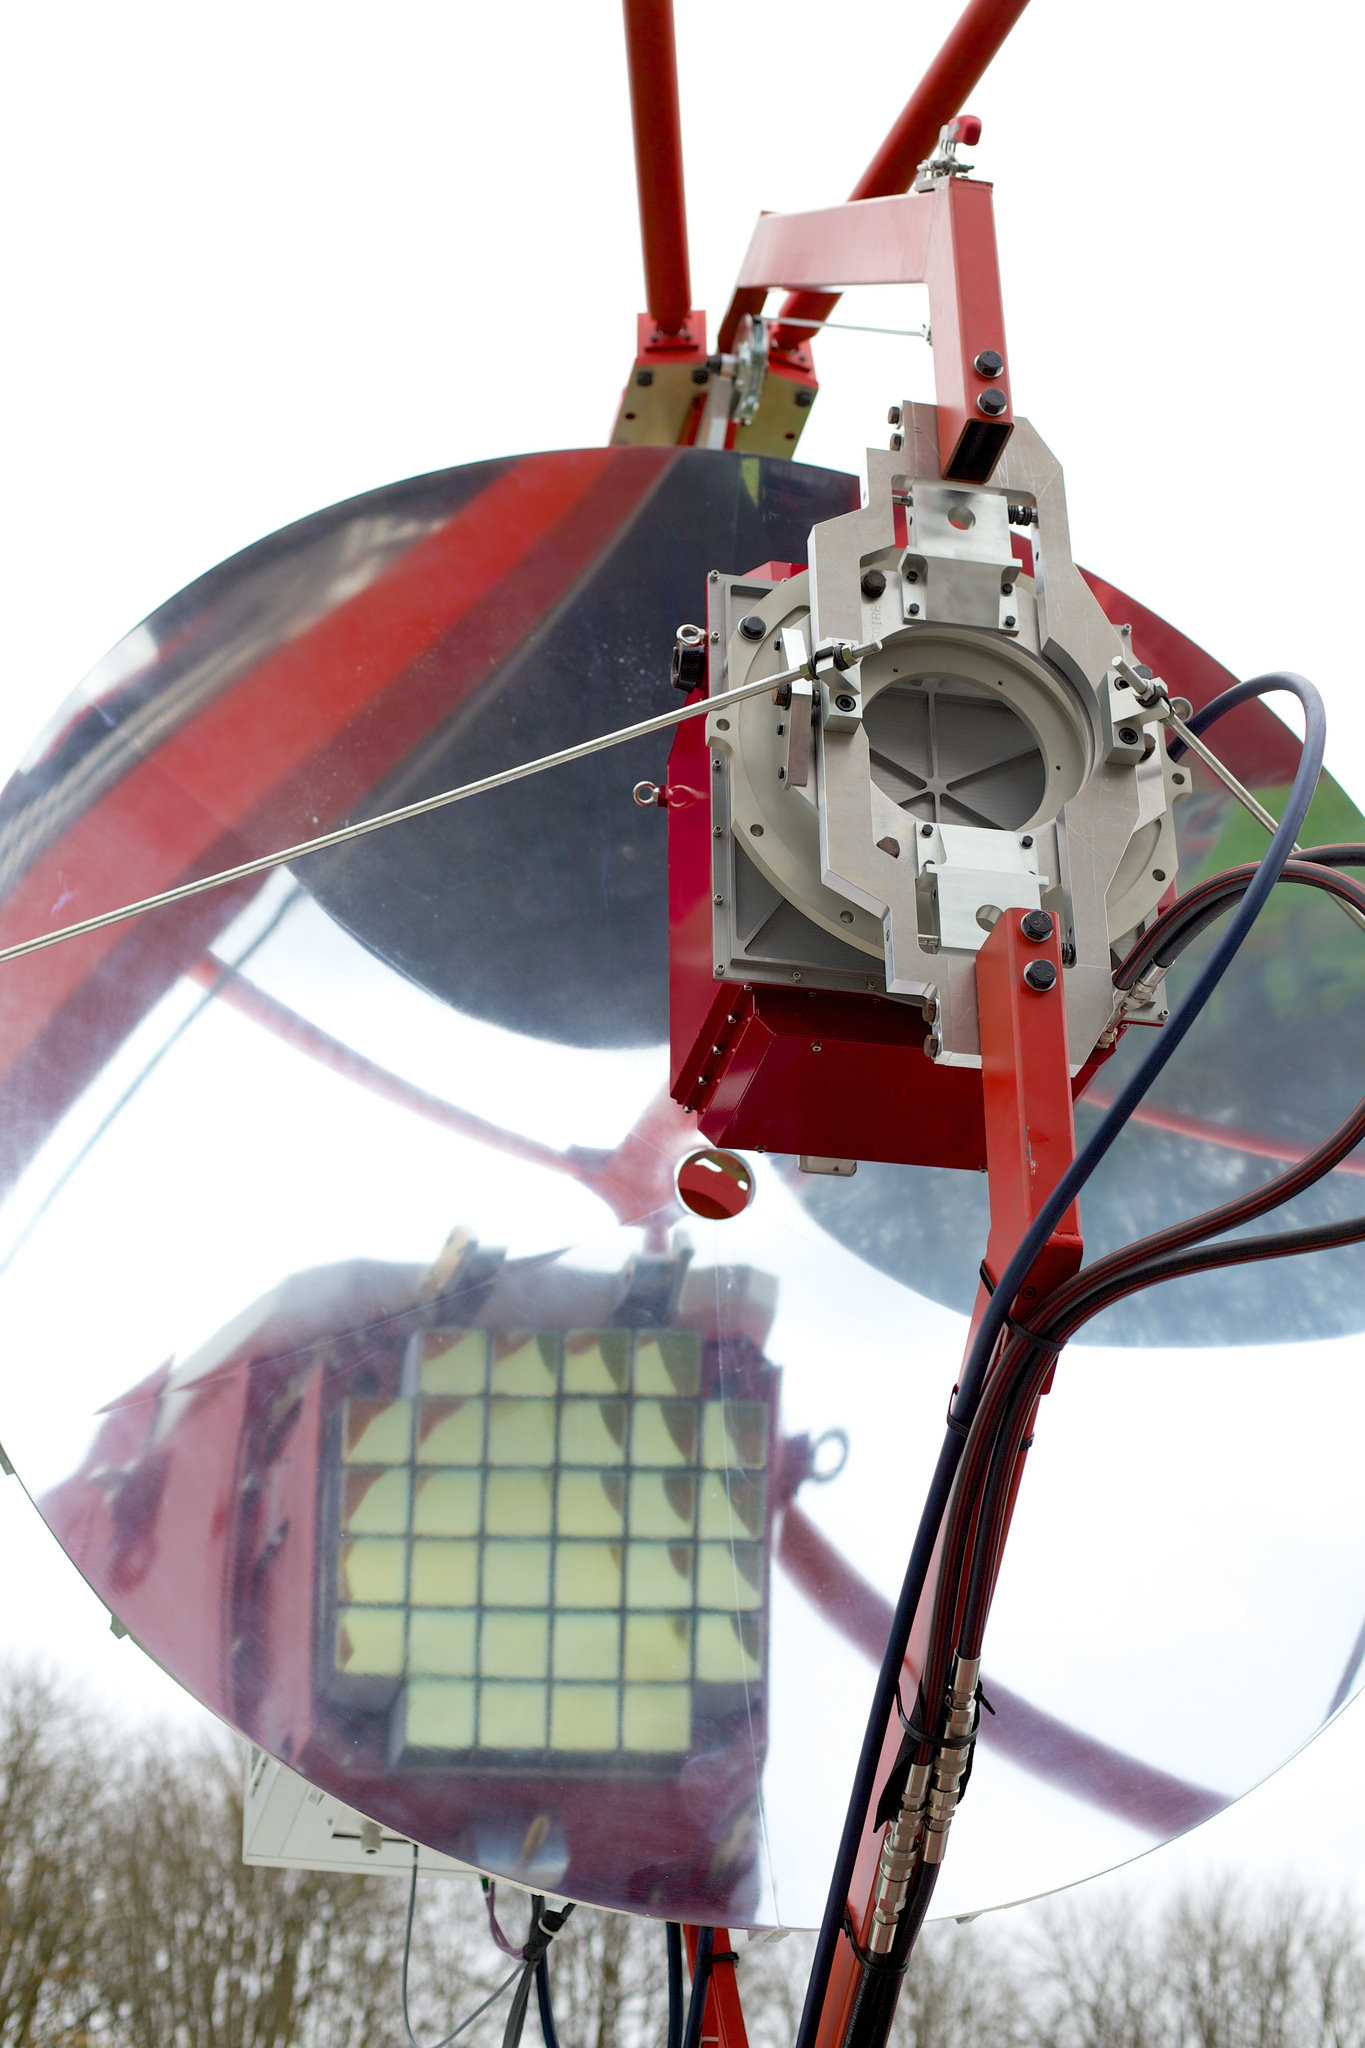
\includegraphics[width=0.6\textwidth]{akira-reflection}
  \caption[Photo of the reflection of CHEC-M in the secondary mirror.]{Photo of the reflection of CHEC-M in the GCT telescope's secondary mirror, taken during the first on-telescope campaign \cite{akira-reflection}.}
  \label{fig:akira-reflection}
\end{figure}

Testing the operation of the camera on the telescope structure is a very important part of the commissioning procedure. When on-telescope, the camera is in an environment we have very little control over. It is exposed to factors such as weather conditions and excessive \gls{nsb} from various sources (including moonlight, starlight, and artificial light pollution). The on-telescope campaigns are therefore a useful measure of the robustness of the camera, and the procedures used to operate the the telescope as a whole.

The first on-telescope campaign took place during November 2015, at the location of the \gls{gct} prototype telescope structure (Observatoire de Paris-Meudon), just before the inauguration of the \gls{gct} prototype. The primary intention of this campaign was to test the integration and operation procedure for \gls{chec-m} on the telescope structure, however the first detection of Cherenkov light from atmospheric showers by a \gls{cta} prototype camera was also achieved \cite{Watson2017}. 

After returning to the lab for further testing and characterisation, \gls{chec-m} was then re-installed on the \gls{gct} structure in March 2017 for a second on-telescope campaign. During this second campaign the \gls{gct} telescope was pointed towards two \gls{vhe} gamma-ray sources, Mrk421 and Mrk501. These two sources are blazar objects (\gls{agn} with a relativistic jet directed towards Earth) and were the first extragalactic \si{TeV} sources to be discovered \cite{Punch1992, Quinn1996} \final{fix Quinn}, testifying to their brightness. However, due to the high \gls{nsb} background that is present at the Meudon site due to it proximity to Paris (20 to 100 times higher \gls{nsb} than expected at the final \gls{cta} site), the camera had to be operated at a low gain and high trigger threshold \cite{Zorn2017}. The former setting was used as a precaution to avoid damage to the \glspl{mapmt}, and the latter to avoid triggering on the \gls{nsb} photons. The combination of these operating conditions, and the limited observation time, meant an astrophysical detection was unlikely for this campaign. Nevertheless, Cherenkov showers were detected during the campaign. This chapter will describe the results I have obtained from the camera images taken during the campaign.

\section{Cherenkov Shower Images}

Utilising the calibration procedure defined in Chapter~\ref{ch5-calibration}, and a simple integration window combined with the \textit{Neighbour Peak Finding} technique described in Chapter~\ref{ch6-reduction}, the signal in each pixel was extracted for every trigger event. The results shown in this section originate from a 30-minute-long observation of Mrk501, during which the camera received triggers at a rate of \SI{\sim 0.1}{Hz}.

\begin{figure}
  \centering
  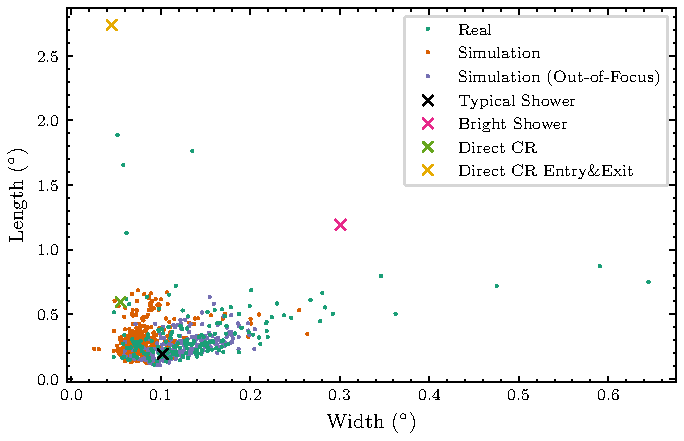
\includegraphics[width=\textwidth]{hillas_checm_width_length}
  \caption[\textit{Hillas} length versus width for an on-sky observation run with CHEC-M.]{The \textit{Hillas} length versus width of each image in a 30-minute-long observation of Mrk501 with CHEC-M on the \gls{gct} telescope structure (labelled as ``Real''). Simulations of CHEC-M on the \gls{gct} telescope are also included for comparison. Four different types of events have been highlighted and assigned a category based on a manual examination of their camera image.}
  \label{fig:hillas_checm_width_length}
\end{figure}

\begin{sidewaysfigure}
  \begin{subfigure}[b]{0.49\textwidth}
    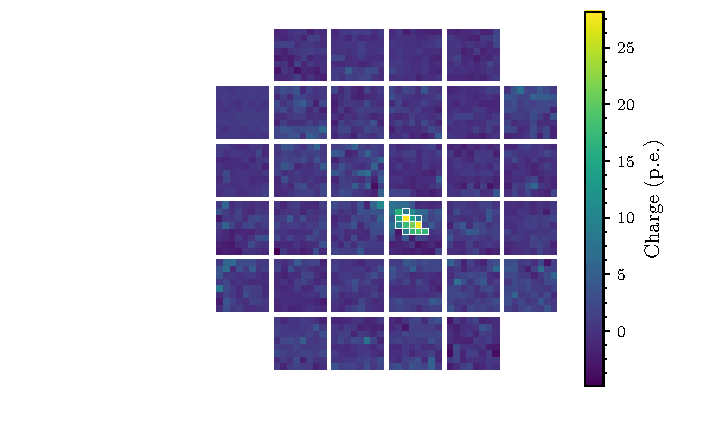
\includegraphics[width=\textwidth]{hillas_checm_typical}
    \caption{Typical Shower}
    \label{fig:hillas_checm_typical}
  \end{subfigure}
  \hfill
  \begin{subfigure}[b]{0.49\textwidth}
    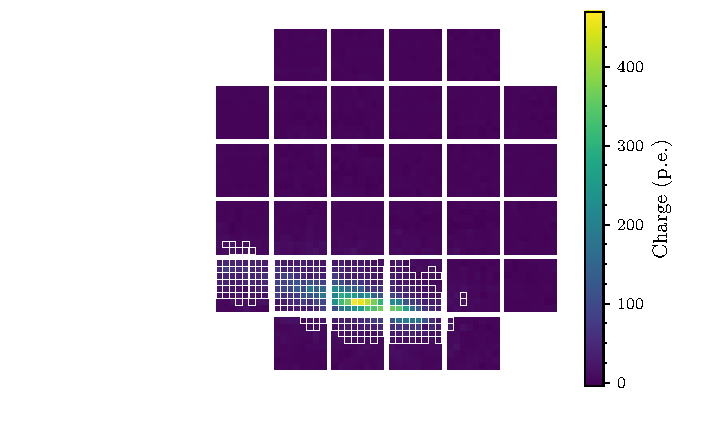
\includegraphics[width=\textwidth]{hillas_checm_bright}
    \caption{Bright Shower}
    \label{fig:hillas_checm_bright}
  \end{subfigure}
   \hfill
  \begin{subfigure}[b]{0.49\textwidth}
    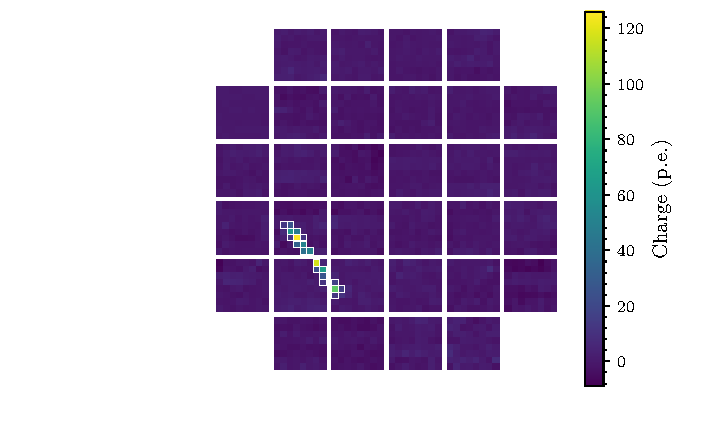
\includegraphics[width=\textwidth]{hillas_checm_cr}
    \caption{Direct CR}
    \label{fig:hillas_checm_cr}
  \end{subfigure}
  \hfill
  \begin{subfigure}[b]{0.49\textwidth}
    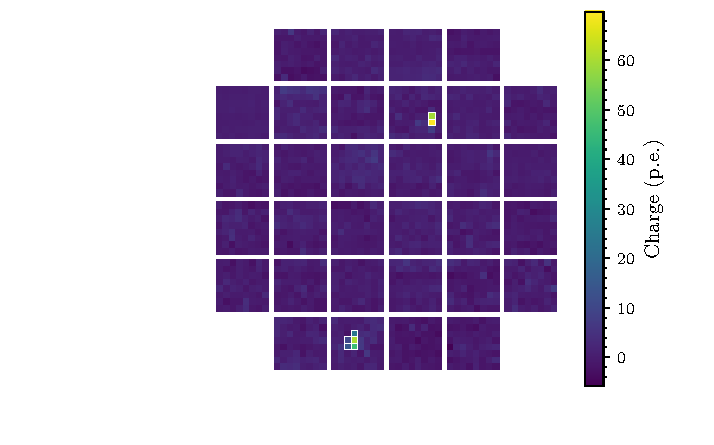
\includegraphics[width=\textwidth]{hillas_checm_cr_ee}
    \caption{Direct CR Entry\&Exit}
    \label{fig:hillas_checm_cr_ee}
  \end{subfigure}
  \caption[Selection of on-sky images.]{A selection of images taken by \gls{chec-m} during its second on-telescope campaign. The images chosen correspond to the individually highlighted events in Figure~\ref{fig:hillas_checm_width_length}.}
  \label{fig:checm_cherenkov_images}
\end{sidewaysfigure}

Figure~\ref{fig:hillas_checm_width_length} displays the distribution of \textit{Hillas} width and length (Section~\ref{section:image_parametrisation}) for the events that caused a camera trigger. Four events were chosen from the collection, and are marked with a cross on the figure. The images corresponding to each of the selected events are shown in Figure~\ref{fig:checm_cherenkov_images}. These events were manually selected as they represent a range of possible event types:
\begin{itemize}
\item Figure~\ref{fig:hillas_checm_typical} - A typical Cherenkov shower, most likely produced from a hadronic cosmic ray due to their abundance compared to gamma-ray showers. The majority of events fall under this category, and result in a cluster at low values of \textit{Hillas} width and length.
\item Figure~\ref{fig:hillas_checm_bright} - A bright Cherenkov shower, from a high energy cosmic ray. These events are characterised by their large \textit{Hillas} width and length. 
\item Figure~\ref{fig:hillas_checm_cr} - A direct cosmic ray, grazing along the pixels on the focal surface and producing an electron avalanche in the \glspl{mapmt}. As the signal is located along the incident path of the cosmic ray, the ratio of \textit{Hillas} length to width for these events is large. Due to their locality to a single telescope, these events are ignored in an \gls{iact} array, as only a single telescope triggers.
\item Figure~\ref{fig:hillas_checm_cr_ee} - Another cosmic ray. Due to the curved focal surface of \gls{chec-m}, it is possible for a cosmic ray to enter and exit the focal surface at opposite sides. These events are characterised by very large ratios of \textit{Hillas} length to width.
\end{itemize}

A Monte Carlo simulation of proton-induced Cherenkov showers, combined with a model of \gls{chec-m} on the \gls{gct} telescope structure, was produced for a comparison against the real results. The signal and Hillas parameters were extracted from the simulated waveforms, with the identical procedures used for the real data. The distribution of \textit{Hillas} width and length are also shown in Figure~\ref{fig:hillas_checm_width_length}, under the label ``Simulation''. It is immediately apparent that the distribution of \textit{Hillas} width is a lot tighter in the simulation. An explanation for this is supplied later in Section~\ref{section:onsky_conclusion}.

\section{Jupiter Observations}

\begin{figure}
  \centering
  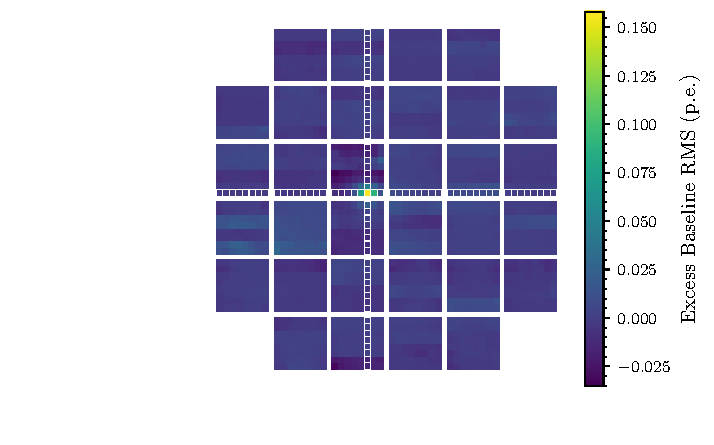
\includegraphics[width=\textwidth]{jupiter_image}
  \caption[Camera image of the excess baseline RMS for observations of Jupiter.]{Camera image of the excess baseline RMS for observations of Jupiter taken during the second on-telescope campaign for CHEC-M.}
  \label{fig:jupiter_image}
\end{figure}

\begin{figure}
  \begin{subfigure}[b]{0.49\textwidth}
    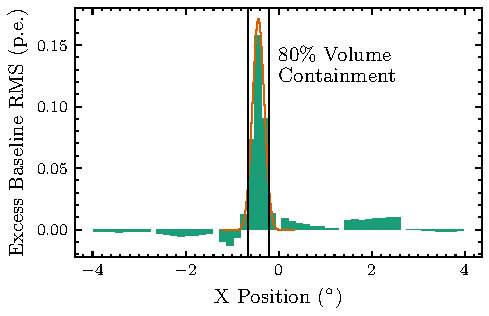
\includegraphics[width=\textwidth]{jupiter_1d_projection_x}
    \caption{Slice along the X axis.}
    \label{fig:jupiter_1d_projection_x}
  \end{subfigure}
  \hfill
  \begin{subfigure}[b]{0.49\textwidth}
    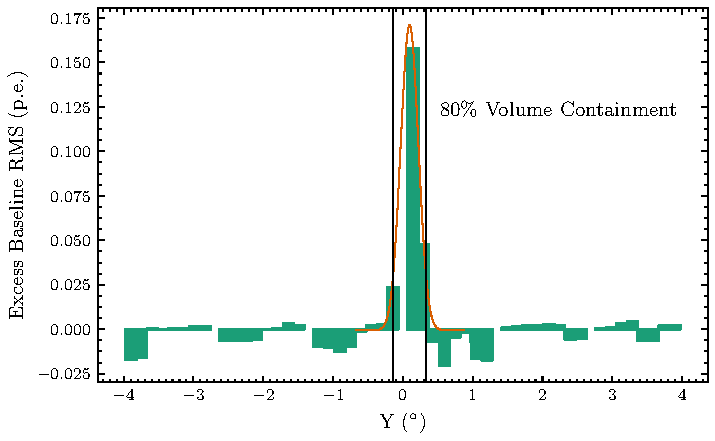
\includegraphics[width=\textwidth]{jupiter_1d_projection_y}
    \caption{Slice along the Y axis.}
    \label{fig:jupiter_1d_projection_y}
  \end{subfigure}
  \caption[Camera slices of the Jupiter observations.]{Slices of the camera image from Figure~\ref{fig:jupiter_image}, along the white-highlighted pixels, showing the excess baseline RMS from each pixel in the slice. A slice of the 2D Gaussian fit to the PSF resulting from observing Jupiter is also shown, along with the corresponding \SI{80}{\percent} volume containment radius.}
  \label{fig:jupiter_1d_projection}
\end{figure}

\begin{figure}
  \centering
  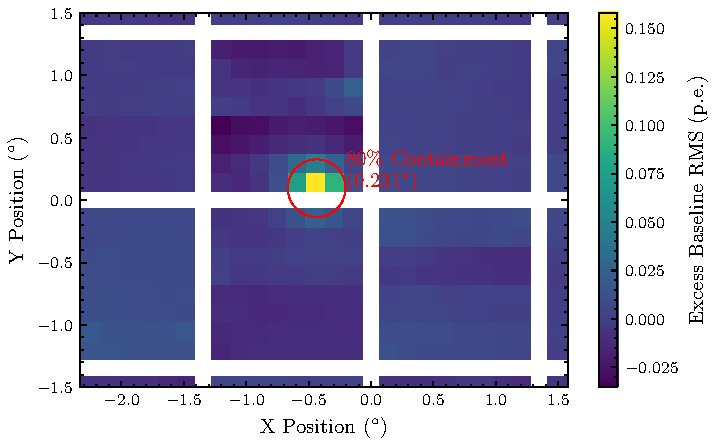
\includegraphics[width=\textwidth]{jupiter_contour}
  \caption[Zoom of the Jupiter camera image.]{Zoom of Figure~\ref{fig:jupiter_image}, showing the result of the 2D Gaussian fit to the PSF resulting from observing Jupiter, and the corresponding \SI{80}{\percent} containment radius.}
  \label{fig:jupiter_contour}
\end{figure}

It has been considered within \gls{cta} that the pointing calibration for the telescopes may be performed using the change in pixel current as a star crosses a pixel's boundary \cite{Gaug2014}. As one of the primary effects of a higher \gls{nsb} (such as that from starlight) is the increased variation of the waveform's baseline, it may be possible to achieve a pointing calibration using this information instead of the currents. An initial investigation into this possibility was explored during the second on-telescope campaign using Jupiter as a source.

Two runs were taken: an ``ON'' axis observation, and an ``OFF'' axis observation. The ON observation was pointed at (and tracked) Jupiter, however intentionally slightly off axis to avoid it being located in the gap at the centre of the camera. The OFF observation was taken without Jupiter, or any other optically bright star in the \gls{fov}. The camera was triggered externally triggered at a rate of \SI{300}{Hz} for approximately 5 minutes. This resulted in approximately 80,000 waveforms per pixel for each of the observations. The \gls{rms} of the waveforms was extracted for each waveform, and averaged over all events. The average \gls{rms} per pixel for the OFF observations were then subtracted from the ON observations. This removed any contributions from the camera electronics. 

The resulting camera image of the excess \gls{rms} per pixel is shown in Figure~\ref{fig:jupiter_image}. This profile of Jupiter in the camera is a measure of the \gls{psf} of the telescope. The value that is used in \gls{cta} to characterise the \gls{psf} is the \SI{80}{\percent} containment radius \cite{Armstrong2015,Rulten2016}. To extract this value, a 2D Gaussian was fit to the camera image, using the X and Y coordinates of every pixel and their corresponding value of excess \gls{rms} baseline. In Figures~\ref{fig:jupiter_1d_projection_x}~and~\ref{fig:jupiter_1d_projection_y}, a slice of the camera image for each axis is shown, intersecting at the pixel with the maximum excess RMS. Shown alongside the pixels distributions are the corresponding slices of the 2D Gaussian fit, demonstrating the fit's successful representation of the profile, event with it being on the edge of a module. Figure~\ref{fig:jupiter_contour} illustrates the \SI{80}{\percent} containment radius radius on the camera image, resulting in a value of \SI{0.23}{\degree}. 

\section{Conclusion} \label{section:onsky_conclusion}

The value extracted for the \gls{psf} is a magnitude larger than expected from Monte Carlo simulations, where a value of \SI{\sim 0.02}{\degree} was obtained \cite{Armstrong2015}. This result is compatible with the discrepancy seen in the \textit{Hillas} width between the real observations and simulations in Figure~\ref{fig:hillas_checm_width_length}. One possible source of this discrepancy is the quality of the prototype mirrors. As shown by \textcite{Rulten2016}, an increase in the mirror surface roughness translates into an increase in the \gls{psf}. A second potential explanation is an incorrect separation between the camera focal plane. It was concluded by \textcite{Rulten2016} that an a incorrect separation of just a few millimetres could account for a magnitude increase in the \SI{80}{\percent} containment value. 

A new simulation was generated with a \gls{psf} of \SI{0.28}{\degree}, to more closely represent the \gls{psf} of the telescope prototype. The \textit{Hillas} parameter distribution we obtain from this simulation, labelled as ``Simulation (Out-of-Focus)'' in Figure~\ref{fig:hillas_checm_width_length}, is in much closer agreement with the \textit{Hillas} parameters obtained during the on-telescope campaign. 

\section{Future}

The next on-telescope campaign is planned for November 2018, where \gls{chec-s} will be placed on the \gls{astri} telescope structure which has been constructed on Mt. Etna, Sicily \cite{Maccarone2017}. This will be the first on-telescope campaign for the \gls{chec-s} prototype, and the first time a \gls{chec} prototype has been installed on the \gls{astri} telescope structure. This campaign will extend for two weeks, during which priority will be given to the characterisation of the trigger efficiency in the presence of \gls{nsb}, and the formalisation of the operation procedures. New Cherenkov shower detections will also be obtained during this campaign, however the detection of a astrophysical gamma-ray source is not a priority of the campaign.